\documentclass[12pt,a4paper]{article}
\usepackage[utf8]{inputenc}
\usepackage[T1]{fontenc}
\usepackage{amsmath}
\usepackage{amssymb}
\usepackage{makeidx}
\usepackage{graphicx}
\usepackage[italian]{babel}
\usepackage{float}
\usepackage{listings}
\usepackage{color}
\definecolor{dkgreen}{rgb}{0,0.6,0}
\definecolor{gray}{rgb}{0.5,0.5,0.5}
\definecolor{mauve}{rgb}{0.58,0,0.82}

\lstset{frame=tb,
	language=SQL,
	aboveskip=3mm,
	belowskip=3mm,
	showstringspaces=false,
	columns=flexible,
	basicstyle={\small\ttfamily},
	numbers=none,
	numberstyle=\tiny\color{gray},
	keywordstyle=\color{blue},
	commentstyle=\color{dkgreen},
	stringstyle=\color{mauve},
	breaklines=true,
	breakatwhitespace=true,
	tabsize=3
}

\title{Tesi di Laurea}
\author{}
\begin{document}
	\begin{titlepage}
		
		\begin{center}
			
			\textsc{\LARGE Università degli Studi di Trieste}\\[0.25cm] 
			\textsc{\large Dipartimento di Ingegneria e Architettura}\\[2.0cm] 
			
			{\large	Tesi di Laurea Triennale in:}\\[0.25 cm]
			{\large \bfseries INGEGNERIA ELETTRONICA E INFORMATICA}
			\\[2 cm]
			{\large  EXTENDED SUMMARY OF: }\\[0.25cm]
			{\large \bfseries CDR-MAC: A Protocol for Full
				Exploitation of}\\ [0.2 cm]
			{\large \bfseries Directional Antennas
				in Ad Hoc Wireless Networks
}\\[1.0cm]
			
			
			\vfill
			%\includegraphics[width=1\textwidth]{images/report_front}\par
			
				\begin{table}[h]
					{\large
						\begin{tabular}{c c c c l c c c c r}
							Laureando: & & & & & & & &  Relatore: \\
							\bfseries Alessandro Di Santo & & & & & & & &   \bfseries Comisso Massimiliano 
						\end{tabular}
					}
				\end{table}
			
			
				
			
			~
		
			
		
			\vspace{.1\linewidth}
			
			\rule{.4\textwidth}{.10pt}
			\\[0.2 cm]
			
				{\large \par	
					Anno Accademico: 2024/2025\\
					\par}
				
			
			
		\end{center}
	\end{titlepage}
\newpage
\tableofcontents
\newpage

\section{Introduzione}

	Si vuole realizzare una base di dati per una società che lavora con i concessionari di automobili, con lo scopo di organizzare e gestire i dati delle aziende.
	
	
\subsection{Requisiti della Base di Dati}

	I concessionari sono identificati da un codice, un nome e dalla città in cui operano. Ogni concessionario possiede un autosalone e un’officina, pertanto svolge sia l’azione di vendita che di riparazione.
	\\
	\\
	Per ogni automobile in vendita è necessario sapere la targa, il modello, il prezzo, la carrozzeria (suv, cabrio, berlina) e il tipo di carburante che utilizza (benzina, diesel, elettrica). Un’automobile può essere una supercar oppure una citycar, e può essere acquistata solo dai clienti possessori di patente sportiva o patente normale, rispettivamente. 
	\\
	\\
	Il cliente può rivolgersi a un concessionario sia per una riparazione (di cui evidenzieremo la data) sia per l’acquisto di un’automobile (di cui evidenzieremo la data). Del cliente ci interessa sapere il nome, il cognome, l’indirizzo (via, cap, civico) e l’età. Il cliente è in possesso di un conto corrente (numero e saldo) e potrebbe guidare già un’auto che vorrebbe riparare.
	\\
	\\
	Dell’auto del cliente è necessario conoscere la targa, il guasto, il modello e l’anno.
	\\
	\\
	Ad ogni concessionario attribuiamo la gestione di una cassa di cui ci interessa sapere l’importo. 
	\\
	\\
	Lavorano in ogni concessionario degli impiegati di cui è necessario conoscere la matricola, il nome e il cognome.
\pagebreak
\subsection{Osservazioni}
	Per semplicità consideriamo che se un cliente possiede un’auto allora voglia ripararla (non esiste il caso in cui possegga un’auto e ne voglia acquistare un'altra). Tutti i clienti hanno un conto corrente, mentre solo parte di essi ha un’auto. I clienti che hanno un’auto e quindi voglio farla riparare, posseggono comunque un conto corrente che non utilizzeranno.

\section{Operazioni}
\vspace{5mm}
\begin{itemize}
	\item Resoconto dei profitti (obiettivo stagionale 100.000)
	\begin{flushright}(1 volta ogni 3 mesi) \end{flushright}
	\item Presentare un elenco delle macchine elettriche disponibili
	\begin{flushright}(1 volta ogni mese) \end{flushright}
	\item Presentare un catalogo dei modelli disponibili con i loro rispettivi prezzi
	\begin{flushright}(1 volta ogni 3 mesi) \end{flushright}
	\item Fornire un elenco degli impiegati assunti ed evidenziare il direttore di ogni concessionario
	\begin{flushright}(1 volta all'anno) \end{flushright}

\end{itemize}


\section{Schema Entity-Relationship}
\vfill
\begin{figure}[H]
	\centering
	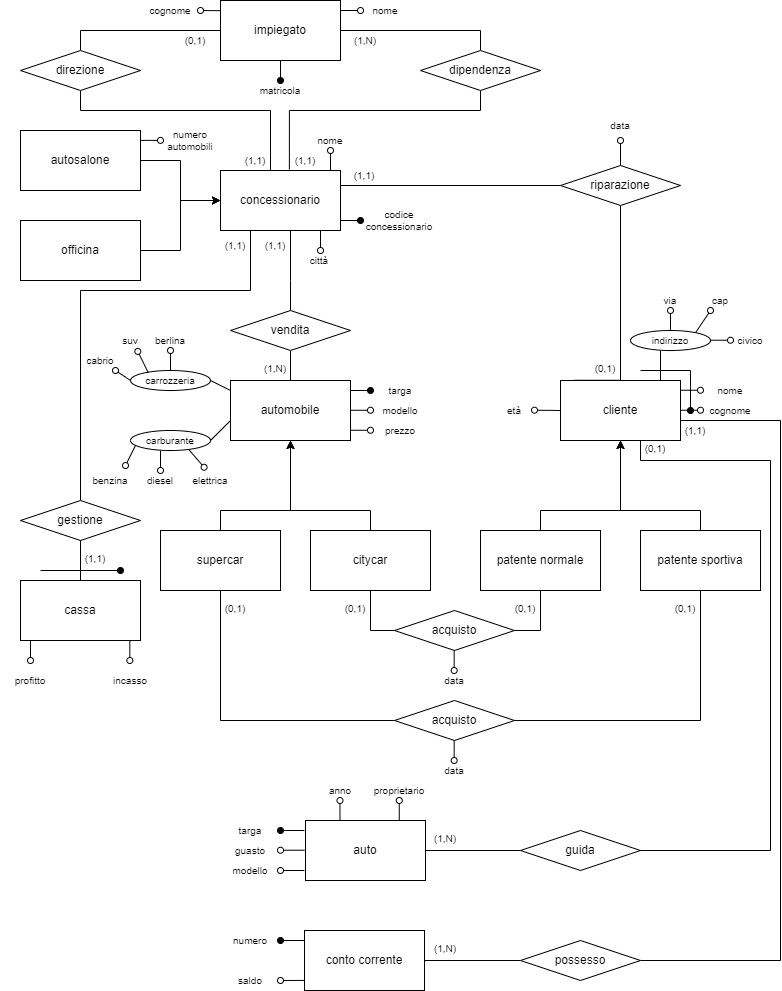
\includegraphics[width=1.1\textwidth]{immagini/E-R}
	
\end{figure}
\vfill

\section{Dizionario dei Dati}
\begin{itemize}
	\item Dizionario delle Entità
\end{itemize}
\begin{figure}[H]
	\centering
\begin{tabular}{|c|p{40mm}|p{40mm}|p{30mm}|}
	\hline
	\textbf{Entità} & \textbf{Descrizione}  & \textbf{Attributi} & \textbf{Identificatore} \\
	\hline
	Impiegato & Colui che lavora per un concessionario (può essere anche il direttore) & Matricola, nome, cognome  &  Matricola \\
	\hline
	Concessionario & Azienda che vende e ripara automobili  & Codice concessionario, nome, città, numero automobili &  Codice concessionario  \\
	\hline
	Automobile & Oggetto in vendita presso un concessionario & Targa, modello, anno, prezzo, carrozzeria, carburante & Targa \\
	\hline
	Cliente  & Colui che si rivolge al concessionario per comprare o per farsi riparare l’auto & Codice cliente, nome, cognome, indirizzo, età & Codice cliente \\
	\hline
	Conto corrente & Conto in possesso del cliente & Numero di conto, saldo & Numero di conto \\
	\hline
	Auto & Automobile in possesso del cliente & Targa, guasto, modello, anno, proprietario & Targa  \\
	\hline
	Cassa & Deposito del denaro incassato da un concessionario & Incasso, profitto & Gestione (R)\\
	\hline
\end{tabular}
\end{figure}

\pagebreak
\begin{itemize}
	\item Dizionario delle Relazioni
\end{itemize}
\begin{figure}[H]
	\centering
\begin{tabular}{|c|p{40mm}|p{40mm}|p{30mm}|}
	\hline
	\textbf{Relazione} & \textbf{Descrizione}  & \textbf{Componenti} & \textbf{Attributi} \\
	\hline
	Direzione & Direzione da parte di un impiegato (il direttore) di un concessionario & Impiegato, concessionario &  \\
	\hline
	Dipendenza & Dipendenza degli impiegati che lavorano per un concessionario & Impiegato, concessionario &  \\
	\hline
	Vendita & Vendita delle automobili & Concessionario, automobile  & \\
	\hline
	Riparazione & Riparazione da parte del concessionario delle auto del cliente & Concessionario, cliente & Data  \\
	\hline
	Guida  &  Macchine in possesso al cliente &  Cliente, auto &  \\
	\hline
	Possesso & Conto corrente di cui dispone il cliente & Cliente, conto corrente &  \\
	\hline
	Acquisto & Acquisto di un’automobile da parte del cliente & Cliente, automobile & Data \\
	\hline
	Gestione & Gestione da parte del concessionario della propria cassa  & Concessionario, cassa &  \\
	\hline
\end{tabular}
\end{figure}

\vspace{5mm}
\section{Vincoli non esprimibili graficamente}

\begin{itemize}
	\item Si possono riparare solo le auto con un anno > 2015
	\item Possono possedere una patente solo i clienti con un età >= 18
	\item Solo uno degli attributi: "Berlina", "Suv, "Cabrio" può essere diverso da FALSE
	\item Solo uno degli attributi: "Elettrica", "Benzina", "Diesel" può essere diverso da FALSE
	\item L'officina ripara una macchina alla volta 
	
\end{itemize}

\section{Tabella dei Volumi}
	Suppongo che la società per cui è realizzato questo database controlli 50 concessionari.\\
	\\
	Ogni concessionario possiede 200 automobili e ha 30 impiegati, di cui uno è il direttore.\\
	\\
	Si stima una media di 250 clienti l’anno per ogni concessionario, di cui 100 per acquistare un’automobile e 150 per ripararla. Ogni cliente possiede un conto corrente, mentre solo 150 guidano una macchina.\\
	\\
	Si stima che in media ogni cliente che guida una macchina, ne possegga 2.\\
	\\
	Si stima che in media ogni cliente abbia un solo conto corrente.\\
	\\
\begin{figure}[H]
	\centering
\begin{tabular}{|c|c|c|}
	\hline
	\textbf{Concetto} & \textbf{Tipo} & \textbf{Volume} \\
	\hline
	Concessionario& E & 50 \\
	\hline
	Dipendenza & R & 50 \\
	\hline
	Impiegato & E & 1500 (=30$\cdot$50) \\
	\hline
	Direzione & R & 50 \\
	\hline
	Vendita & R & 50 \\
	\hline
	Automobile & E & 10000 (=50$\cdot$200) \\
	\hline
	Riparazione & R & 50 \\
	\hline
	Cliente & E & 12500 (=(100+150)$\cdot$50) \\
	\hline
	Acquisto & R & 5000 (=100$\cdot$50) \\
	\hline
	Guida & R & 7500 (=150$\cdot$50) \\
	\hline
	Auto & E & 15000 (=7500$\cdot$2) \\
	\hline
	Possesso & R & 12500 \\
	\hline
	Conto Corrente & E & 12500 \\
	\hline
	Gestione & R & 50 \\
	\hline
	Cassa & E & 50 \\
	\hline
\end{tabular}

\end{figure}

\section{Schema Entity-Relationship Ristrutturato}
\vfill
\begin{figure}[H]
	\centering
	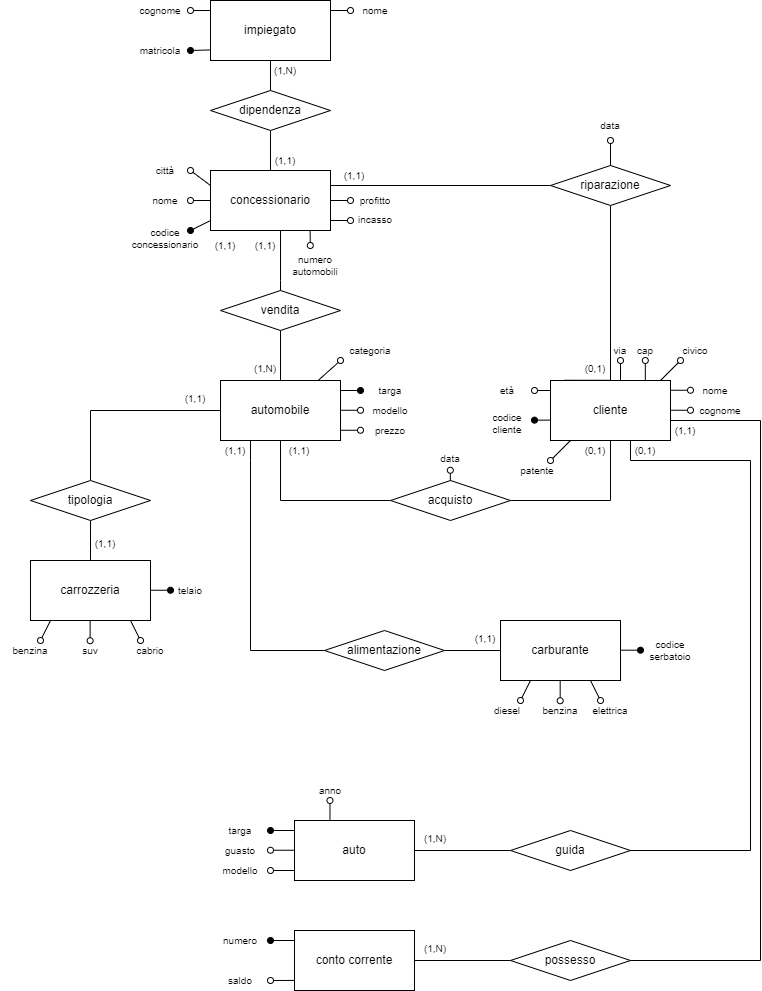
\includegraphics[width=1.1\textwidth]{immagini/E-R.ristrutturato}
	
\end{figure}
\vfill

\subsection{Eliminazione Generalizzazioni}
	
	Per quanto riguarda le entità automobile e cliente, sono state eliminate entrambe le generalizzazioni, scegliendo di accorpare i figli al genitore, e fondendo le due relazioni che univano le specializzazioni. Esse diventano così degli attributi “categoria” nell’entità automobile e “patente” nell’entità cliente. Questa scelta implica l’inserimento di un vincolo (Trigger) che permette le relazioni solo tra entità in cui l’attributo “categoria” corrisponde con “patente”.\\
	\\
	Per quanto riguarda l’entità concessionario, è stata eliminata la generalizzazione accorpando i figli al genitore, ovvero le specializzazioni “autosalone” e “officina”.
	

\subsection{Analisi Ridondanze}

	L’entità “auto” presenta l’attributo “proprietario” che risulta calcolabile dalla relazione “guida” con il cliente. Decidiamo, pertanto, di eliminare tale attributo calcolabile.\\
	\\
	L’entità “concessionario” presenta un altro attributo calcolabile attraverso la funzione count(), cioè “numero automobili”. Si è deciso, però, date le operazioni da svolgere, di mantenere l’attributo ridondante per migliorare le prestazioni del database.\\
	\\
	Notiamo che è presente un ciclo tra “concessionario”, “automobile” e “cliente”, questo crea ridondanza siccome possiamo intuire dal cliente che acquista un’auto che non voglia ripararla, e viceversa. Tuttavia, trattandosi di due operazioni differenti svolte dal concessionario si è preferito non eliminare tale ciclo.\\
	\\
	Un altro ciclo si viene a creare tra “impiegato” e “concessionario”, in questo caso abbiamo una ridondanza, perché se un impiegato è dipendente del concessionario, posso ricavare che non è il direttore. Possiamo eliminare tale ciclo associando al direttore di un dato concessionario l’attributo “matricola”=1. Nell’operazione che porta alla presentazione dell’elenco degli impiegati verrà evidenziato il direttore di ogni concessionario.

\pagebreak
\subsection{Eliminazione Attributi Composti}

	Tutti gli attributi composti sono stati scorporati in attributi semplici.

\subsection{Partizionamento}
\begin{itemize}
	\item \textbf{Partizionamento delle Entità}\\
	\\
	Siccome abbiamo eliminato gli attributi composti presenti nell’entità automobile si è deciso di eseguire un partizionamento di essa in due nuove entità: “carrozzeria” e “carburante” collegate dalle relazioni “tipologia” e “alimentazione”, rispettivamente, all’entità automobile.
	\item \textbf{Partizionamento delle Relazioni}\\
	\\
	Non è necessario partizionare nessuna relazione.
\end{itemize} 
\subsection{Accorpamento}
\begin{itemize}
	\item \textbf{Accorpamento delle Entità}\\
	\\
	In quanto relazione (1,1) e siccome attributi di concetti diversi a cui accediamo contemporaneamente si è deciso di eseguire un accorpamento di entità tra: “concessionario” e “cassa”. Avremo, pertanto, due nuovi attributi nell’entità concessionario, ovvero: “profitto” e “incasso”.
	\item \textbf{Accorpamento delle Relazioni}\\
	\\
	Siccome abbiamo eliminato le specializzazioni di Automobile e Cliente, dovremo eseguire un accorpamento delle relazioni Acquisto in una sola.
\end{itemize} 
\pagebreak
	
\subsection{Scelta Identificatori Primari}
Sono stati aggiunti degli identificatori nell’entità “carrozzeria” e “carburante” che rispettino i criteri richiesti: assenza di opzionalità, semplicità e utilizzo nelle operazioni più frequenti.
 
 \begin{itemize}
 	\item \textbf{Impiegato}: si decide di utilizzare come identificatore l’attributo “Matricola”
 	\item \textbf{Concessionario}: si decide di utilizzare come identificatore l’attributo “Codice Concessionario”
 	\item \textbf{Automobile}: si decide di utilizzare come identificatore l’attributo “Targa”
 	\item \textbf{Carrozzeria}: si decide di utilizzare come identificatore l’attributo “Telaio”
 	\item \textbf{Carburante}: si decide di utilizzare come identificatore l’attributo “Codice Serbatoio”  
 	\item \textbf{Cliente}: si decide di utilizzare come identificatore l’attributo “Codice Cliente”
 	\item \textbf{Auto}: si decide di utilizzare come identificatore l’attributo “Targa”
 	\item \textbf{Conto Corrente}: si decide di utilizzare come identificatore l’attributo “Numero di Conto”
 	
 \end{itemize} 
\pagebreak
 
\subsection{Passaggio al Modello Relazionale}
\begin{itemize}
	\item \textbf{Concessionario} (\underline{Codice concessionario}, Nome, Città, Numero automobili, Profitto, Incasso, Data, Impiegato, Automobile, Cliente)
	\begin{itemize}
		\item integrità referenziale tra impiegato e matricola
		\item integrità referenziale tra automobile e targa
		\item integrità referenziale tra cliente e codice cliente
	\end{itemize}
	\item \textbf{Impiegato} (\underline{Matricola}, Nome, Cognome)
	\item \textbf{Automobile} (\underline{Targa}, Modello, Prezzo, Categoria, Carrozzeria, Carburante)
	\item \textbf{Cliente} (\underline{Codice Cliente}, Patente, Via, CAP, Civico, Nome, Cognome, Età, Data, Automobile, Auto, Conto Corrente)
	\begin{itemize}
		\item integrità referenziale tra automobile e targa
		\item integrità referenziale tra auto e targa
		\item integrità referenziale tra conto corrente e numero di conto
	\end{itemize}
	
	\item \textbf{Conto Corrente} (\underline{Numero conto}, saldo)
	\item \textbf{Auto} (\underline{Targa}, Guasto, Modello, Anno)
	\begin{itemize}
		\item integrità referenziale tra carrozzeria e telaio
		\item integrità referenziale tra carburante e codice serbatoio
	\end{itemize}
	\item \textbf{Carrozzeria} (\underline{Telaio}, Berlina, Suv, Cabrio)
	\item \textbf{Carburante} (\underline{Codice Serbatoio}, Diesel, Benzina, Elettrica)
	
\end{itemize}

	
\section{Schema Logico}
\vfill
\begin{figure}[H]
	\centering
	\includegraphics[width=0.65\textwidth]{immagini/Schema_logico}
\end{figure}
\vfill
\pagebreak
\subsection{Normalizzazione}
\begin{itemize}
	\item La base di dati è già in \textbf{prima forma normale}, dato che tutte le colonne sono atomiche.\\
	
	\item La base di dati è già in \textbf{seconda forma normale}, siccome ogni colonna dipende dalla chiave primaria.\\

	\item Per quanto riguarda la \textbf{terza forma normale}, possiamo notare che non è soddisfatta dal nostro database, siccome sono presenti dei campi calcolati nelle tabelle: Carrozzeria e Carburante. 
	\begin{itemize}
		\item Analizziamo la tabella Carrozzeria, per quella Carburante varranno le stesse considerazioni. Notiamo, infatti, che il valore dell'attributo Berlina può essere intuito non solo dalla PK, ma anche dal valore degli attributi: Suv e Cabrio. Per ovviare a tale problema, invece di creare un tabella ulteriore (detta tabella di lookup), siccome in tal caso rimarrebbe la tabella Carrozzeria munita della sola PK; si potrebbero cambiare gli attributi calcolati evidenziati in precedenza, con un singolo attributo: \begin{lstlisting}
			TipoCarrozzeria CHAR(1)
		\end{lstlisting} 
		oppure
		\vspace{2mm}
		\begin{lstlisting}
			TipoCarrozzeria VARCHAR(10)
		\end{lstlisting} 
		In realtà si potrebbe eliminare del tutto l'entità Carrozzeria e accorparla nell'entità Automobile. In precedenza, però, è stato eseguito un partizionamento per una comprensione migliore del database; quindi in virtù dei vincoli imposti e per le ragioni presentate, si è deciso di non portare avanti tale soluzione.\\
	\end{itemize}
	
\end{itemize}

	
\pagebreak
\section{Realizzazione Base di Dati}
\begin{lstlisting}
CREATE DATABASE IF NOT EXISTS ConsulenzaConcessionario;
USE ConsulenzaConcessionario;

CREATE TABLE Concessionario (
	CodiceConcessionario INT AUTO_INCREMENT,
	Nome VARCHAR(45) NOT NULL,
	Citta VARCHAR(45) NOT NULL,
	NumeroAutomobili INT NOT NULL,
	Profitto INT NOT NULL,
	Incasso INT NOT NULL,
	Data CHAR(10),
	Impiegato INT,
	Automobile INT(7),
	Cliente INT,
	PRIMARY KEY (CodiceConcessionario),
	FOREIGN KEY (Impiegato) REFERENCES Impiegato(Matricola),
	FOREIGN KEY (Automobile) REFERENCES Automobile(Targa),
	FOREIGN KEY (Cliente) REFERENCES Cliente(CodiceCliente)
);

CREATE TABLE Impiegato (
	Matricola INT AUTO_INCREMENT,
	Nome VARCHAR(45) NOT NULL,
	Cognome VARCHAR(45) NOT NULL,
	PRIMARY KEY (Matricola)
);

CREATE TABLE ContoCorrente (
	NumeroConto INTEGER AUTO_INCREMENT,
	Saldo INTEGER NOT NULL,
	PRIMARY KEY(NumeroConto)
);

CREATE TABLE Cliente (
	CodiceCliente INT AUTO_INCREMENT,
	Nome VARCHAR(45) NOT NULL,
	Cognome VARCHAR(45) NOT NULL,
	Patente BOOL,
	Via VARCHAR(50) NOT NULL,
	Civico TINYINT NOT NULL,
	Cap CHAR(2) NOT NULL,
	Eta INT NOT NULL,
	Auto INT(7),
	Data CHAR(10),
	ContoCorrente INT,
	PRIMARY KEY (CodiceCliente),
	FOREIGN KEY (Auto) REFERENCES Auto(Targa),
	FOREIGN KEY (ContoCorrente) REFERENCES ContoCorrente(NumeroConto)
);

CREATE TABLE Automobile (
	Targa CHAR(7),
	Modello VARCHAR(45) NOT NULL,
	Prezzo INT NOT NULL,
	Categoria BOOL NOT NULL,
	Carrozzeria INT(17),
	Carburante INT(20),
	PRIMARY KEY (Targa),
	FOREIGN KEY (Carrozzeria) REFERENCES Carrozzeria(Telaio),
	FOREIGN KEY (Carburante) REFERENCES Carburante(CodiceSerbatoio)
);

CREATE TABLE Auto (
	Targa INT(7) AUTO_INCREMENT,
	Guasto VARCHAR(200) NOT NULL,
	Modello VARCHAR(45) NOT NULL,
	Anno CHAR(4) NOT NULL,
	PRIMARY KEY (Targa)
);

CREATE TABLE Carrozzeria (
	Telaio INT(17) AUTO_INCREMENT,
	Berlina BOOL NOT NULL,
	Suv BOOL NOT NULL,
	Cabrio BOOL NOT NULL,
	PRIMARY KEY (Telaio)
);

CREATE TABLE Carburante (
	CodiceSerbatoio INT(20) AUTO_INCREMENT,
	Diesel BOOL NOT NULL,
	Benzina BOOL NOT NULL,
	Elettrica BOOL NOT NULL,
	PRIMARY KEY (CodiceSerbatoio));


\end{lstlisting}
\newpage
\section{Realizzazione delle Operazioni}
Resoconto dei profitti (obiettivo stagionale 100.000) (stored procedure).
\begin{lstlisting}
	DELIMITER$$
	CREATE PROCEDURE profitti
	(
		IN codice_concessionario INT,
		OUT tot_profitti INT
	)
	BEGIN
		SELECT Profitto INTO tot_profitti
		FROM Concessionario 
		WHERE CodiceConcessionario=codice_concessionario;
		IF tot_profitti>100000 THEN
			SIGNAL SQLSTATE '45001' SET MESSAGE_TEXT= 'Obiettivo raggiunto';
		ELSE
			SIGNAL SQLSTATE '45002' SET MESSAGE_TEXT ='Obiettivo non raggiunto';
		END IF;
	END $$
	DELIMITER;
\end{lstlisting}

$\,$\\[0.5cm]
Numero di macchine elettriche disponibili per un dato concessionario (stored procedure).
\begin{lstlisting}
	DELIMITER$$
	CREATE PROCEDURE numeroElettriche
	(
		IN codice_concessionario INT,
		INOUT tot_elettriche INT
	)
	BEGIN
		DECLARE finished INT DEFAULT 0;
		DECLARE i BOOL;
		DECLARE cursore CURSOR FOR SELECT c.Elettrica 
		FROM Carburante c
		LEFT JOIN Automobile a
		ON c.CodiceSerbatoio=a.Carburante
		LEFT JOIN Concessionario co
		ON a.Targa=co.CodiceConcessionario
		WHERE co.CodiceConcessionario=codice_concessionario;
		DECLARE CONTINUE HANDLER FOR NOT FOUND SET finished=1;
		SET tot_elettriche=0;
		OPEN cursore;
		WHILE (finished=0) DO
			FETCH cursore INTO i;
			IF finished=0 THEN
				IF i=TRUE THEN
					SET tot_elettriche=tot_elettriche+1;
				END IF;
			END IF;
		END WHILE;
		CLOSE cursore;
	END $$
	DELIMITER;
	
	\end{lstlisting}

$\,$\\[0.5cm]
Catalogo dei modelli disponibili con i rispettivi prezzi  (stored procedure).
\begin{lstlisting}
	DELIMITER$$
	CREATE PROCEDURE catalogoAuto
	(
		IN codice_concessionario INT,
		OUT lista_modelli VARCHAR(10000)
	)
	BEGIN
		DECLARE finished INT DEFAULT 0;
		DECLARE modelli VARCHAR(250) DEFAULT " ";
		DECLARE cursore CURSOR FOR 
		SELECT a.Modello, a.Prezzo 
		FROM Automobile a
		INNER JOIN Concessionario c
		ON a.Targa=c.Automobile
		WHERE c.CodiceConcessionario = codice_concessionario;
		DECLARE CONTINUE HANDLER FOR NOT FOUND SET finished=1;
		OPEN cursore;
		WHILE(finished=0) DO
			FETCH cursore INTO modelli;
				IF finished=0 THEN
					SET lista_modelli=CONCAT(cursore, ";",lista_modelli);
				END IF;
		END WHILE;
		CLOSE cursore;
	END $$
	DELIMITER;
	
\end{lstlisting}

$\,$\\[0.5cm]
Elenco degli impiegati di un dato concessionario (store procedure).
\begin{lstlisting}
	DELIMITER$$
	CREATE PROCEDURE elenco_impiegati
	(
		IN codice_concessionario INT,
		INOUT numero_impiegati INT,
		INOUT direttore VARCHAR(100)
	)
	BEGIN
		SELECT i.Matricola, i.Nome, i.Cognome, c.CodiceConcessionario FROM Impiegato i
		LEFT JOIN Concessionario c
		ON i.Matricola=c.Impiegato
		WHERE c.CodiceConcessionario=codice_concessionario;
		IF i.Matricola=1 THEN
			SET direttore=CONCAT(i.Nome," ",i.Cognome," ",c.CodiceConcessionario);
		END IF;
	
		SELECT count(*) INTO numero_impiegati
		FROM Impiegato
		WHERE Matricola IN (
			SELECT Impiegato 
			FROM Concessionario 
			WHERE CodiceConcessionario=codice_concessionario);
	END $$
	DELIMITER;
	
\end{lstlisting}


\newpage
\section{Realizzazione dei Vincoli}
Si possono riparare solo le auto con un anno > 2015 (trigger)
\begin{lstlisting}
	DELIMITER$$
	CREATE TRIGGER controllo_anno
	AFTER UPDATE OF Anno ON Auto
	FOR EACH ROW 
	BEGIN
		IF new.Anno<=2015 THEN
			SIGNAL SQLSTATE '45003' SET MESSAGE_TEXT = 'Auto troppo vecchia per essere riparata';
		END IF;
	END $$
	DELIMITER;
	
\end{lstlisting}

$\,$\\[0.5cm]
Possono avere la patente, e di conseguenza acquistare o riparare una macchina, solo i clienti che hanno un’età >= 18 anni (trigger)
\begin{lstlisting}
	DELIMITER $$
	CREATE TRIGGER controllo_eta
	AFTER UPDATE OF Eta ON Cliente
	FOR EACH ROW
	BEGIN
		IF new.Eta<18 THEN
			SIGNAL SQLSTATE '45004' SET MESSAGE_TEXT = 'Il cliente in questione non ha la patente';
		END IF;
	END $$
	DELIMITER;
\end{lstlisting}

$\,$\\[0.5cm]
Solo uno degli attributi: “berlina”, “suv” e “cabrio” può essere diverso da FALSE (trigger)
\begin{lstlisting}
	DELIMITER $$
	CREATE TRIGGER controlloCarrozzeria
	AFTER UPDATE ON Carrozzeria
	FOR EACH ROW
	BEGIN
		IF NEW.Berlina=TRUE AND (NEW.Suv=TRUE OR NEW.Cabrio=TRUE) THEN
			SIGNAL SQLSTATE '45004' SET MESSAGE_TEXT = 'Impossibile non solo berlina=TRUE';
		ELSEIF NEW.Suv = TRUE AND (NEW.Berlina = TRUE OR NEW.Cabrio = TRUE) THEN
			SIGNAL SQLSTATE '45005' SET MESSAGE_TEXT = 'Impossibile non solo suv=TRUE';
		ELSEIF NEW.Cabrio = TRUE AND (NEW.Berlina = TRUE OR NEW.Suv = TRUE) THEN
			SIGNAL SQLSTATE '45006' SET MESSAGE_TEXT = 'Impossibile non solo cabrio=TRUE';
		END IF;
	END $$
	DELIMITER ;
\end{lstlisting}


$\,$\\[0.5cm]
Solo uno degli attributi: “diesel”, “benzina” ed “elettrica” può essere diverso da FALSE (trigger)
\begin{lstlisting}
	DELIMITER $$
	CREATE TRIGGER controlloCarburante
	AFTER UPDATE ON Carburante
	FOR EACH ROW
	BEGIN
		IF NEW.Elettrica = TRUE AND (NEW.Benzina = TRUE OR NEW.Diesel = TRUE) THEN
			SIGNAL sqlstate '45201' SET MESSAGE_TEXT = 'Impossibile non solo elettrica=TRUE';
		ELSEIF NEW.Diesel = TRUE AND (NEW.Elettrica = TRUE OR NEW.Benzina = TRUE) THEN
			SIGNAL sqlstate '45202' SET MESSAGE_TEXT = 'Impossibile non solo diesel=TRUE';
		ELSEIF NEW.Benzina = TRUE AND (NEW.Elettrica = TRUE OR NEW.Diesel = TRUE) THEN
			SIGNAL sqlstate '45203' SET MESSAGE_TEXT = 'Impossibile non solo benzina=TRUE';
		END IF;
	END $$
	DELIMITER;
\end{lstlisting}

\pagebreak
$\,$\\[0.5cm]
Trigger che permette le relazioni solo tra entità in cui l’attributo “categoria” corrisponde con “patente”
\begin{lstlisting}
	DELIMITER$$
	CREATE TRIGGER controlloPatenteCliente
	AFTER UPDATE ON Cliente, Automobile
	FOR EACH ROW
	BEGIN
		IF NEW.Patente<>NEW.Categoria THEN
			SIGNAL SQLSTATE '45007' SET MESSAGE_TEXT = "La patente del cliente non corrisponde con la categoria di auto che puo' acquistare";
		END IF;
	END $$
	DELIMITER;
\end{lstlisting}

$\,$\\[0.5cm]
Quando passiamo al cliente successivo vuol dire che, se prima c'è stata una riparazione, il guasto del cliente precedente è stato sanato (trigger)
\begin{lstlisting}
	$$DELIMITER
	CREATE TRIGGER tr_guasto
	BEFORE UPDATE ON Cliente
	FOR EACH ROW
	BEGIN
		IF OLD.Auto IS NOT NULL THEN
			UPDATE Auto
			SET Guasto = 'Auto riparata'
			WHERE Targa = OLD.Auto;
		END IF;
	END $$
	DELIMITER;
	
\end{lstlisting}

\end{document}